\documentclass[11pt]{article}
\usepackage[margin=0.98in]{geometry}
\usepackage{amsmath,amssymb,booktabs}
\usepackage{graphicx}
\usepackage[expansion=false]{microtype}
\usepackage[font=small,labelfont=bf,skip=4pt]{caption}
\usepackage[colorlinks=true,linkcolor=black,citecolor=black,urlcolor=blue]{hyperref}
\usepackage{titlesec}
\titlespacing{\section}{0pt}{0.95em}{0.35em}
\titlespacing{\subsection}{0pt}{0.8em}{0.3em}
\setlength{\parskip}{0.22em}
\renewcommand{\topfraction}{0.92}
\renewcommand{\bottomfraction}{0.75}
\renewcommand{\textfraction}{0.06}
\renewcommand{\floatpagefraction}{0.85}
\newcommand{\rs}{$r^{*}$}
\begin{document}
\begin{center}
{\large\textbf{Disagreement in \boldmath$r^{*}$?}}\\[0.3em]
\end{center}
\vspace{0.1em}
\noindent\rule{\textwidth}{0.4pt}
\suppressfloats[t]
\vspace{0.2em}
% =====================================================================
\section{The question}
Long-term bond yields are anchored by beliefs about where short rates settle in the long run. A revision to that endpoint passes into the yield at every maturity, undamped by horizon, in a way that news about the current policy stance does not. This is why the endpoint has been at the center of the term-structure literature since Kozicki and Tinsley's shifting endpoints, and why Bauer and Rudebusch's falling stars put a slow-moving anchor at the heart of it. What is unsettled is where those beliefs come from, and whether the central bank is one of the sources.
Consider a policy rule written as follows,
\begin{equation}
i_t \;=\; \underbrace{r^{*}_t + \pi^{*}_t}_{\text{intercept}} \;+\; \phi_\pi\!\left(\pi_t - \pi^{*}_t\right) + \phi_x x_t + v_t ,
\label{eq:rule-general}
\end{equation}
\rs{} is the \emph{intercept} of the reaction function, so ``the Fed reveals \rs{}'' means the
Fed is telling markets about the constant in its own rule. Bauer, Pflueger \& Sunderam (2024)
estimate the perceived \emph{slope} $\phi_\pi$ and show it prices term premia; they absorb the
intercept into forecaster fixed effects. The intercept has been assumed
known, assumed common, or differenced away.
\begin{quote}
\textbf{How does the Fed move beliefs about the intercept of its own reaction function, and
what does disagreement about that intercept do to the price of long bonds?}
\end{quote}
\noindent In three parts:
\begin{enumerate}
    \item \textbf{Who moves whom}: Does the FOMC's published longer-run projection move primary dealers' beliefs about the same object, and by how much? And does the dealers' projection, which the Desk reports to the Committee before every meeting, move the FOMC's own, and by how much?
    \item \textbf{Pricing}: Does a revision to the published projection move the yield curve with the maturity profile of an endpoint shock? Can the term-premium response be separated from stance news and from a perceived policy error?
    \item \textbf{Disagreement}: Does dispersion in beliefs about the intercept carry a risk premium whose sensitivity does not decay with maturity? Does a signed Fed-minus-market gap move the level of yields, with the split between breakeven and real-rate responses pinned by the perceived rule?
\end{enumerate}
\clearpage
\section{Decomposing Long Yields}
Start from the definition of a long yield as an average of expected short rates plus a
residual:
\begin{equation}
y^{(n)}_t \;=\; \underbrace{\frac{1}{n}\sum_{j=0}^{n-1} E_t\!\left[i_{t+j}\right]}_{\text{expectations component } rn^{(n)}_t} \;+\; TP^{(n)}_t .
\label{eq:eh}
\end{equation}
Now split the nominal policy rate into a neutral level and a deviation from it. Define the
\emph{neutral nominal rate} and the \emph{policy gap}
\begin{equation}
i^{*}_t \;\equiv\; r^{*}_t + \pi^{*}_t ,
\qquad
\text{gap}_t \;\equiv\; i_t - i^{*}_t \;=\; \underbrace{\left(i_t - E_t\pi_{t+1} - r^{*}_t\right)}_{\text{real policy stance}} \;+\; \underbrace{\left(E_t\pi_{t+1} - \pi^{*}_t\right)}_{\text{inflation deviation}} ,
\label{eq:gapdef}
\end{equation}
where $r^{*}_t$ is the equilibrium real rate and $\pi^{*}_t$ the long-run inflation
anchor. The gap is therefore \textbf{the stance of policy}: how far the Fed is holding the
short rate above or below the level that would be neutral, plus how far inflation is
expected to run from its anchor. Under a Taylor-type rule
$i_t = i^{*}_t + \phi_\pi(\pi_t-\pi^{*}_t) + \phi_x x_t + v_t$, the gap is exactly the
systematic and discretionary response to the cycle,
\begin{equation}
\text{gap}_t \;=\; \phi_\pi\!\left(\pi_t-\pi^{*}_t\right) + \phi_x x_t + v_t .
\label{eq:taylor}
\end{equation}
Substituting \eqref{eq:gapdef} into \eqref{eq:eh}, and adding the martingale assumption for
the endpoints --- $E_t[r^{*}_{t+j}]=r^{*}_t$ and $E_t[\pi^{*}_{t+j}]=\pi^{*}_t$ --- gives
\begin{equation}
y^{(n)}_t \;=\; r^{*}_t \;+\; \pi^{*}_t \;+\; \frac{1}{n}\sum_{j=0}^{n-1} E_t\!\left[\text{gap}_{t+j}\right] \;+\; TP^{(n)}_t .
\label{eq:identity}
\end{equation}
Equivalently, in terms of the neutral nominal rate,
\begin{equation}
y^{(n)}_t \;=\; i^{*}_t \;+\; \frac{1}{n}\sum_{j=0}^{n-1} E_t\!\left[\text{gap}_{t+j}\right] \;+\; TP^{(n)}_t .
\label{eq:identity-istar}
\end{equation}
% From (4) we have that the gap at each time $t$ is equivelent to the Fed's policy response at that time. If the Fed's Policy Response is AR(1) with persistance $\rho$ we further decompose,
% Hillenbrand's evidence that the window decline is not the policy cycle is that it survives in the 5-year, 5-year-forward rate. That argument requires the expected stance to contribute negligibly at long horizons. It does not. The expected-gap term in \eqref{eq:identity} enters the ten-year yield with a weight of roughly 0.5 — estimated from the stance's own dynamics and stable between 0.51 and 0.55 across every specification I fit — so a 100 bp revision to the expected stance moves the ten-year about 50 bp and the 5y5y forward about 30 bp. The far-forward evidence does not separate endpoint news from stance news.
% and over an announcement window,
% \begin{equation}
% \Delta y^{(n)}_t \;=\; \underbrace{\Delta i^{*}_t}_{\text{endpoint news}}
% \;+\; \underbrace{\omega\,\Delta\text{gap}_t + \text{gap}_t\,\Delta\omega}_{\text{stance and persistence news}}
% \;+\; \Delta TP^{(n)}_t .
% \label{eq:windowdiff}
% \end{equation}
\clearpage
% =====================================================================
\section{Three facts}
\subsection{Fact 1: through 2021, yield changes outside FOMC windows net to zero}
% TODO: reconcile 7,035 vs 7,036 non-FOMC day count with results file; regenerate daily SDs
% (5.60/6.72) through the pipeline.
Replicating Hillenbrand (2025) on GSW yields and a hand-built event list: yields move on
non-FOMC days about as much as on FOMC days --- daily standard deviations of 5.60 against
6.72 bp. What differs is that outside the window the moves offset. Across 7{,}035 non-FOMC days
the cumulative change is $-0.82$ pp, a drift of $-0.012$ bp/day with $t = -0.18$; inside
three-day FOMC windows, 11.8\% of trading days, the ten-year fell 6.16 pp of a total 6.99.
Hillenbrand's explanation is \textbf{long-run Fed guidance}: announcements are the moments at
which the Fed reveals its own estimate of where rates settle in the long run --- implicitly
before 2012, when the rate decision itself disclosed the Committee's read of the natural rate,
and explicitly after 2012 through the SEP longer-run dot.
\[
y^{(n)}_t \;=\; i^{*}_t \;+\; \frac{1}{n}\sum_{j=0}^{n-1} E_t\!\left[\text{gap}_{t+j}\right] \;+\; TP^{(n)}_t ,
\]
Hillenbrand's reading is that window moves are $\Delta i^{*}$, which requires the other two
terms to contribute little. For the stance he appeals to the far-forward evidence: the same
downward trend appears in the 5-year, 5-year-forward rate, where the current stance should
long since have washed out. For the term premium he reports in the Internet Appendix that
model-based estimates \emph{do} fall in these windows, and sets the finding aside on the
grounds that those models cannot represent a secular decline. A third result, that the decline
since 1999 is in TIPS rather than breakevens, does not exclude a term but tells us the
composition of $\Delta i^{*}$: it is the real endpoint moving, not the inflation anchor.
\begin{figure}[tbp]
\centering
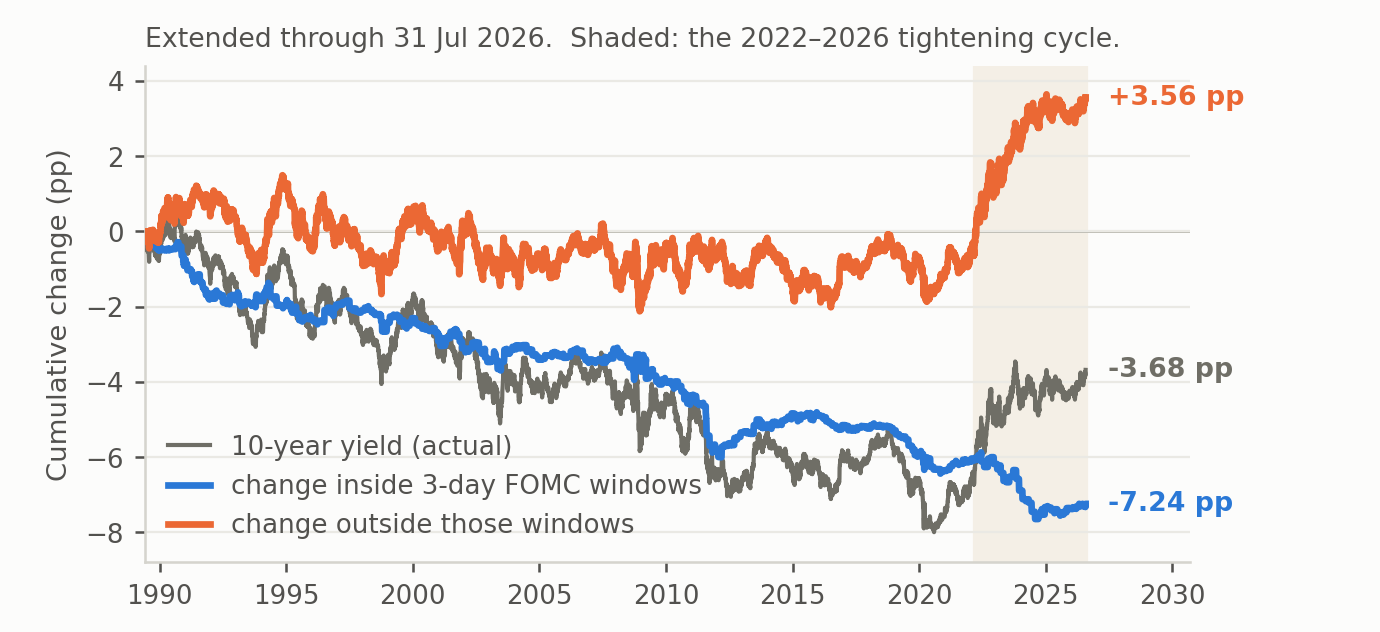
\includegraphics[width=0.78\textwidth]{s_extend.png}
\caption{\textbf{Fact 1.} Cumulative change in the ten-year yield from 2 June 1989, split into
the part accruing inside three-day FOMC windows and the part accruing on all other days.
Shaded: the 2022--2026 tightening cycle.}
\label{fig:fact}
\end{figure}
\subsection{Fact 2: the two beliefs move together, and asymmetrically}
% TODO: state the reverse-regression specification in the text (contemporaneous vs lagged
% dealer revision); the lagged version gave +0.09 (t 1.51). Regenerate 0.31/3.91 and the
% 0.60/0.58 loadings from the results file.
The FOMC publishes its longer-run funds rate projection quarterly; the NY Fed surveys primary
dealers for the same object about two weeks before every meeting. Netting the 2\% objective
from both gives two comparable measures of \rs{} (Figure~\ref{fig:beliefs}). Across 48 matched
meetings (46--47 for the revision regressions): the gap has a standard deviation of
0.105 pp and a range of $-0.11$ to $+0.30$, exceeding 25 bp at 4\% of meetings; dealers move
with the Fed nearly one-for-one ($\beta = 0.82$, $t=6.86$); the reverse relation is present but
weaker ($\beta = 0.31$, $t=3.91$).
\begin{figure}[tbp]
\centering
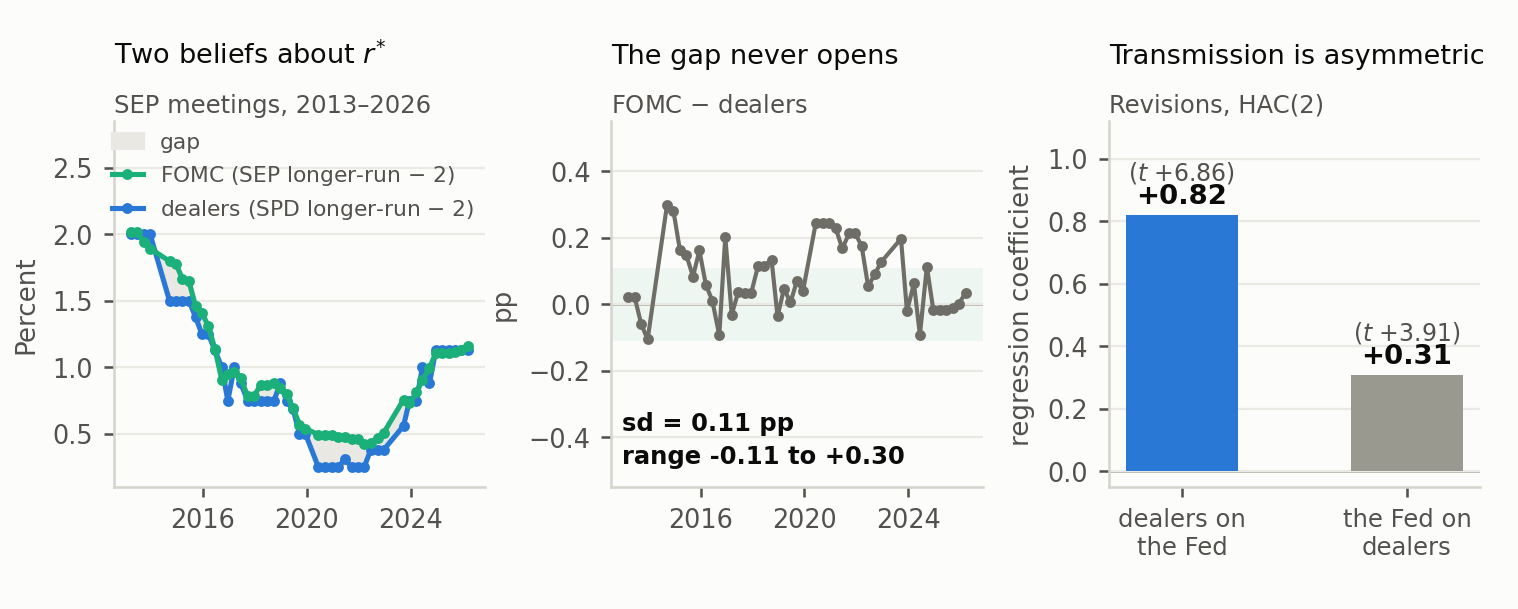
\includegraphics[width=0.82\textwidth]{s_beliefs.png}
\caption{\textbf{Fact 2.} Left: the FOMC's longer-run projection and the primary dealers'
longer-run funds rate, each less 2.0. Centre: the difference. Right: revision regressions,
HAC(2), 46--47 meetings.}
\label{fig:beliefs}
\end{figure}
The asymmetry is not mechanical --- the Desk briefs the FOMC with survey results before each
meeting --- but it is not a clean lead-lag either. Dealer revision loads on
both the preceding dot revision (0.60) and the contemporaneous one (0.58), so part of what looks
like following is anticipation; and intermeeting macro news moves both series, so these
regressions describe timing, not identified transmission. Both series are observed eight times
a year. Section~\ref{sec:tests} adds a pricing counterpart to this fact: the announcement
window prices exactly the part of the dot revision that the dealers' own preceding revision did
not anticipate.
\subsection{Fact 3: the FOMC's $r^{*}$ and the econometric $r^{*}$ move in opposite directions}
% TODO before circulating further: (1) state which HLW code/vintage produced the series;
% (2) re-run on the COVID-adjusted (2023) model; (3) check real-time vintages, which declined
% over 2012-2019; (4) report the revision-level correlation alongside -0.93.
The FOMC's estimate can be compared against the leading model-based alternative. Holston,
Laubach \& Williams estimate the equilibrium real rate from a semi-structural macro model with a
Kalman filter, quarterly from 1961. Under the martingale assumption, these two are estimates of the same object: HLW's contemporaneous
$r^{*}_t$ and the FOMC's longer-run projection coincide when $E_t[r^{*}_{t+j}] = r^{*}_t$.
They do not behave like estimates of the same object (Figure~\ref{fig:rstartwo}). Across the 57
SEP meetings the correlation of levels is $\mathbf{-0.93}$.
Between January 2012 and March 2022 the FOMC marked its own $r^{*}$ \emph{down} by 1.78 pp,
from 2.21\% to 0.42\%, while HLW marked $r^{*}$ \emph{up} by 1.37 pp, from 0.89\% to a peak of
2.26\%. After 2022 they swap: the FOMC revises up 0.74 pp while HLW falls back. The two series
cross exactly once, in June 2016, and the mean absolute gap between them is 0.88 pp --- they sit
within 25 bp of each other at only 5\% of meetings.
\begin{figure}[tbp]
\centering
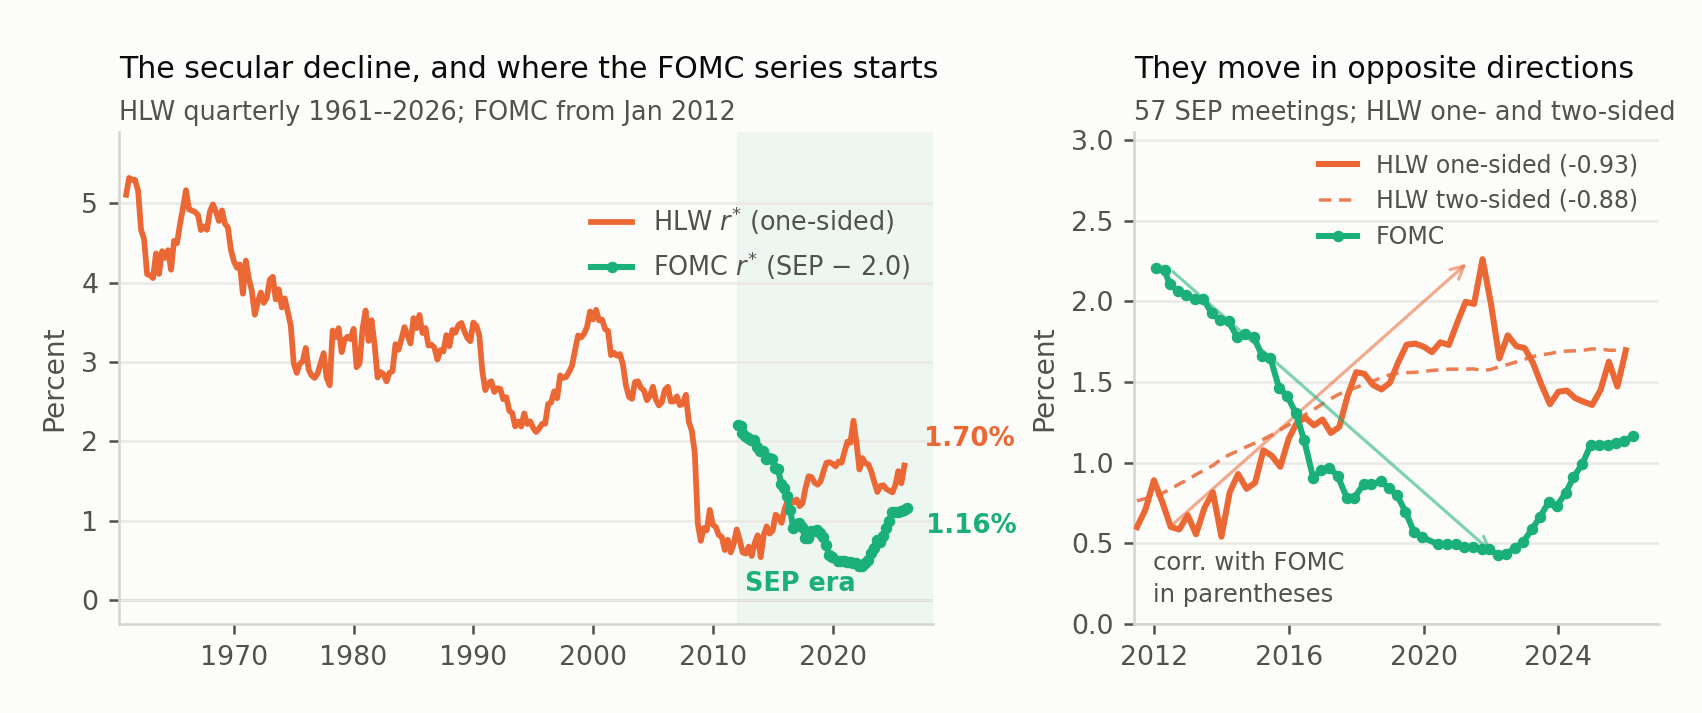
\includegraphics[width=0.95\textwidth]{s_rstar_two.png}
\caption{\textbf{Fact 3.} Left: HLW $r^{*}$ over the full quarterly sample with the FOMC series,
which begins in January 2012, overlaid; the SEP era is shaded. Right: the overlap sample, with
arrows marking the direction each series travels over 2012--2022.}
\label{fig:rstartwo}
\end{figure}
Three things follow. First, the Fed's $r^{*}$ is not easily recoverable from an econometric
model. Second, the same holds for the market side: it is hard to justify a model-based endpoint
to serve as the market perception of $r^*$. Third, the premise that the Fed holds an
information advantage about $r^{*}$ has an observable consequence: over the decade in which the
Committee cut its estimate by 1.78 pp, the filtered econometric estimate moved the other way.
The comparison uses one-sided estimates under current parameters; whether it survives on the
real-time vintages, which declined over 2012--2019, and on the post-COVID revision of the model
is being verified.
One candidate explanation can be rejected immediately. HLW estimates $r^*$ from a model; the
Fed's is inferred from its reported $i^*$ and $\pi^*$, and the SEP reports $\pi^* = 2.0\%$ with
zero variation over the observed sample. If participants report $i^*$ sincerely but hold
$\pi^*$ at 2\% to anchor expectations, the netting $r^{*}_{\text{Fed}} = \text{dot} - 2$ would
mislabel the Fed's real endpoint and the two series would not be comparable.
Figure~\ref{fig:impliedpi} tests this directly: it computes the long-run inflation expectation
that would have to be embedded in the FOMC's projection for the two estimates to agree. That
implied series runs from 3.46\% in September 2012 to 0.20\% in December 2021 --- at its trough
it requires FOMC participants to have expected 0.20\% long-run inflation at a moment when
realised inflation was 5.17\%. Whatever separates the two estimates, it is not the 2\% netting.
\begin{figure}[tbp]
\centering
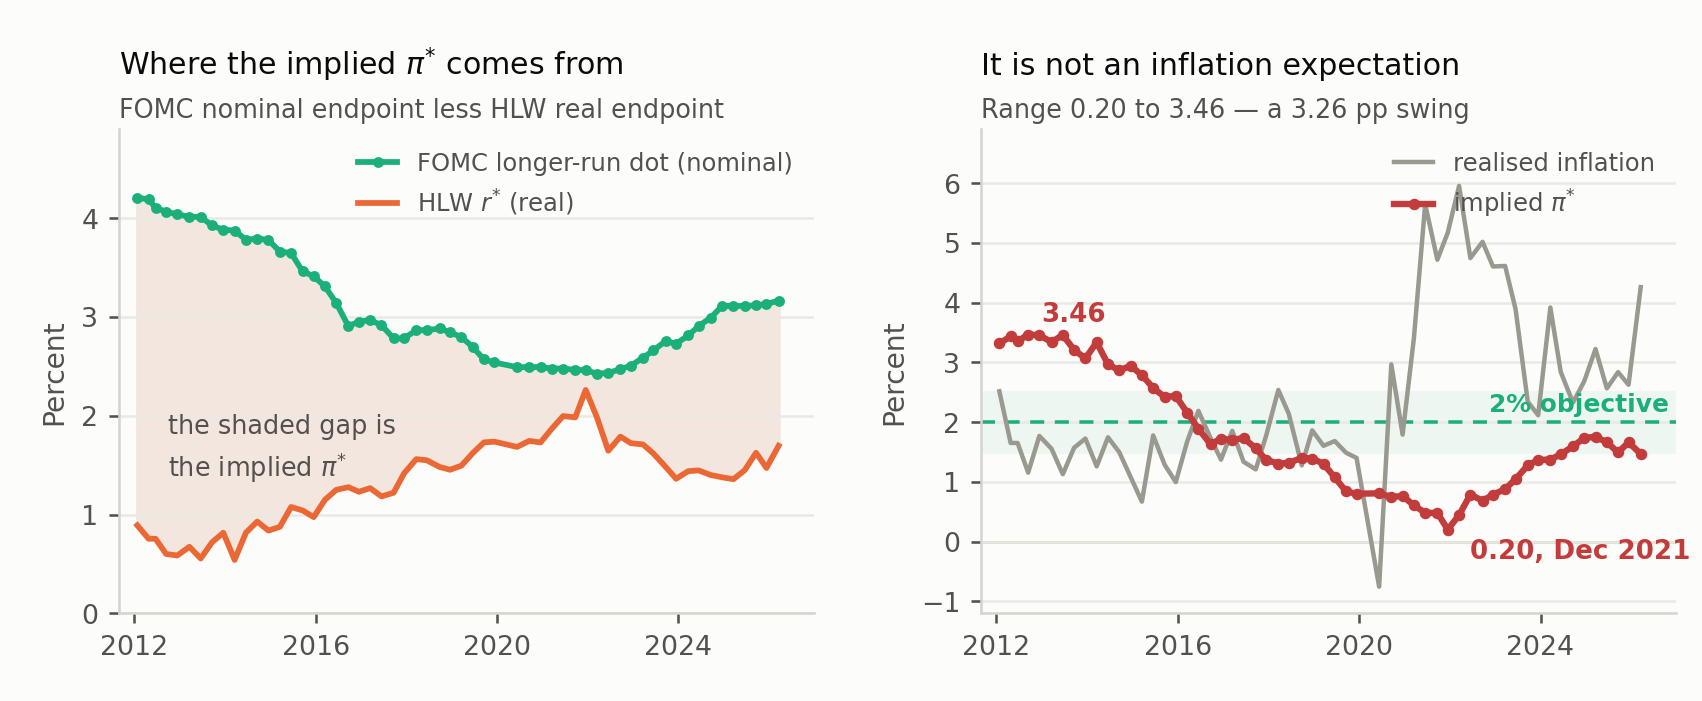
\includegraphics[width=0.95\textwidth]{s_implied_pi.png}
\caption{\textbf{The inflation expectation needed to reconcile the two estimates.} Left: the
FOMC's longer-run federal funds projection, which is nominal, against HLW's one-sided $r^{*}$,
which is real, at the 57 SEP meetings; the shaded area between them is the long-run inflation
expectation that would have to be embedded in the FOMC's projection for the two series to be
mutually consistent. Right: that implied series plotted against realised inflation, with the
2\% objective marked and a 1.5--2.5\% band shaded. The implied series lies outside the
1.5--2.5\% band at 75\% of meetings. Realised inflation is HLW's own four-quarter input series
rather than headline PCE.}
\label{fig:impliedpi}
\end{figure}
% \begin{center}\small
% \begin{tabular}{lrrr}
% \toprule
% Period & bp/meeting & $t$ & Cumulative\\ \midrule
% Jun 1989 -- Dec 2011 (pre-SEP) & $-2.46$ & $-3.06$ & $\mathbf{-5.85}$ pp\\
% Jan 2012 -- Mar 2022 (dot falling 1.78 pp) & $-0.40$ & $-0.41$ & $-0.23$ pp\\
% Mar 2022 -- Jul 2026 (dot rising 0.74 pp) & $-3.49$ & $-1.53$ & $-1.16$ pp\\
% \bottomrule\end{tabular}
% \end{center}
% \noindent 81\% of the in-window decline is complete before the dot plot begins. In the decade
% when the FOMC cut its own longer-run rate by 1.78 pp --- when an information channel should be
% loudest --- the in-window contribution is indistinguishable from zero. Every design using the
% published projection is therefore estimated on a sample in which the motivating phenomenon is
% absent. That is an argument about the whole of Component A, not one contingency within it.
% =====================================================================
\newpage
\section{Framework: intercept disagreement in an opinionated-markets model}
\label{sec:framework}
Caballero \& Simsek (2022) study a Fed and a market that disagree, each confident in its own
view, with the Fed setting policy on its belief and the market pricing assets knowing it will.
The market therefore anticipates policy ``mistakes'' and prices the resulting risk. Their state
variable is aggregate demand. This section runs the same logic with the disagreement located in
the \emph{intercept of the policy rule}. What distinguishes intercept disagreement is not its
persistence --- the estimated Fed--dealer gap mean-reverts with a half-life of about six months
--- but that it maps into a \emph{composition} restriction across the nominal and real curves
that demand disagreement does not generate.
\subsection{Setup}
Both parties know the rule and observe the state. They differ only in the neutral real rate:
the Fed believes $r^{*F}$, the market believes $r^{*m}$, and
\begin{equation}
\delta_t \;\equiv\; r^{*m}_t - r^{*F}_t .
\label{eq:delta}
\end{equation}
The Fed sets policy on its own estimate,
\begin{equation}
i_t \;=\; r^{*F}_t + \pi^{*} + \phi_\pi\!\left(\pi_t - \pi^{*}\right) + \phi_x x_t ,
\qquad \phi_\pi > 1 ,
\label{eq:rule}
\end{equation}
and the market evaluates the resulting stance against \emph{its} neutral rate, perceiving policy
to be $\delta_t$ looser than the Fed intends. Three roles separate whose belief enters where:
\begin{center}\small
\begin{tabular}{@{}lll@{}}
\toprule
& \textbf{Role} & \textbf{Estimate used}\\ \midrule
Fed & Sets $i_t$ through the rule \eqref{eq:rule} & $r^{*F}$\\
Economy & Adjusts $\pi$ until the real rate reaches the natural rate & the truth, $r^{*}$\\
Market & Forecasts the path of $i$; prices bonds off that forecast & $r^{*m}$\\
\bottomrule\end{tabular}
\end{center}
\noindent The market's error is that it substitutes its own $r^{*m}$ for the second row when it
runs the economy forward in its head.
\subsection{The market's subjective steady state}
Consider the steady state the market \emph{forecasts}, holding its belief dogmatically. Two
conditions define it. Over the long run the Fed closes the output gap, so $\phi_x x_t$ drops out
and permanent accommodation is absorbed entirely by inflation rather than output; and the
natural rate is by definition the real rate consistent with a zero gap, so $i-\pi$ equals the
natural rate --- which, in the market's forecast, is the one the market believes in. Setting
$i-\pi = r^{*m}$ in \eqref{eq:rule} gives $(\phi_\pi-1)(\pi-\pi^{*}) = \delta$, so the market
expects inflation to settle permanently away from target at
\begin{equation}
\boxed{\;\pi - \pi^{*} \;=\; \frac{\delta_t}{\phi_\pi - 1}\;}
\label{eq:bias}
\end{equation}
The target is a parameter of the rule, held at 2\% throughout the sample --- all 594 archived
longer-run PCE submissions are exactly 2.0, with zero within-meeting dispersion. What moves is
\emph{realised} long-run inflation. The Fed does not revise its target; it persistently misses
one it continues to hold, because it is setting policy against the wrong intercept. The
adjustment runs through the real rate: at $\pi=\pi^{*}$ the real rate is $r^{*F}$, below the
natural rate, so demand exceeds supply and inflation rises; each point of inflation above target
raises the real rate by $\phi_\pi-1$, until the real rate meets the natural rate. Nobody chooses
the natural rate and nobody chooses $\pi$ --- inflation is the free variable, and it converges
to a finite bias only because $\phi_\pi>1$.
The beliefs are subjective, not actual: in the true steady state $i-\pi=r^{*}$, and
\eqref{eq:bias} with $\delta$ replaced by $r^{*}-r^{*F}$ gives the realised bias, which
coincides with the market's version only if the market happens to be right. Nothing below
requires that it is --- bonds are priced off $E^{m}_t[i_{t+j}]$, so \eqref{eq:bias} and
\eqref{eq:amplification} hold whether or not those expectations are correct. The macro logic is
Orphanides' account of the Great Inflation, a rule fed a mismeasured real-time natural rate
producing a sustained bias, though he locates the mismeasurement in $\phi_x x_t$ where the
mechanism here is in the intercept; Orphanides \& Williams on natural-rate misperception under
learning is the closer antecedent.
\subsection{The amplification result, and what it does and does not identify}
The nominal endpoint the market prices is $r^{*m} + \pi^{*} + \delta/(\phi_\pi-1)$; the endpoint
the FOMC publishes is $r^{*F} + \pi^{*}$. The difference is
\begin{equation}
\boxed{\;\underbrace{i^{*m}_t - i^{*F}_t}_{\text{endpoint gap}} \;=\; \frac{\phi_\pi}{\phi_\pi-1}\;\delta_t\;}
\label{eq:amplification}
\end{equation}
\paragraph{Identification.} The two sides of \eqref{eq:amplification} are distinct objects, and
the distinction is the content of the equation. $\delta$ is disagreement about the \emph{real}
endpoint; the endpoint gap is what that disagreement becomes once the inflation bias it induces
is added to it, $\delta + \delta/(\phi_\pi-1)$, and is larger by the multiplier. So
\eqref{eq:amplification} is one equation in two unknowns, $\delta$ and $\phi_\pi$: the same
observed endpoint gap is consistent with a small disagreement and a weakly-responding perceived
Fed, or a large disagreement and an aggressive one. Recovering $\phi_\pi$ means measuring both
sides independently, and current data supply only one. The SPD's longer-run PCE median is 2.0 in
all 91 surveys, so dealers report a terminal rate that conditions on inflation at target: the
survey delivers $\delta$, not the endpoint gap. Nor can the endpoint gap be taken from prices,
since far-forward risk-neutral rates load heavily on the current short rate. The result is best
read as an identification statement --- the published dot and the market's terminal rate differ
by a \emph{multiple} of the disagreement, and the multiple is the perceived Taylor
coefficient --- independent of the calibration below.
\paragraph{The magnitude claim.} A small disagreement about $r^{*}$ implies a large disagreement
about where nominal rates would settle, with the multiplier set by the perceived $\phi_\pi$:
\begin{center}\small
\begin{tabular}{lccc}
\toprule
$\phi_\pi$ & inflation bias per 1 pp of $\delta$ & endpoint gap per 1 pp of $\delta$ & endpoint gap when sd$(\delta)=0.105$\\ \midrule
1.25 & 4.00 & 5.00 & 52 bp\\
1.50 & 2.00 & 3.00 & 32 bp\\
2.00 & 1.00 & 2.00 & 21 bp\\
2.50 & 0.67 & 1.67 & 18 bp\\
\bottomrule\end{tabular}
\end{center}
\noindent \textbf{These are steady-state numbers}, attained only if the market expects the
disagreement never to be resolved --- and that steady state is self-defeating. Reaching it
requires the Fed to observe inflation running $\delta/(\phi_\pi-1)$ above target indefinitely
--- at $\phi_\pi=1.5$, twice the size of $\delta$ --- and never to revise $r^{*F}$. But a
persistent inflation gap is precisely the signal that identifies an intercept error, so the
mechanism generates the evidence that resolves the disagreement it depends on. That objection is
independent of the estimated persistence and is a reason to expect the permanent component to be
small; the table is an upper bound.
\subsection{The path to the steady state}
\label{sec:path}
The steady-state gap is the limit of a path. Along the market's forecast the inflation bias
builds as the economy responds to the too-low real rate, while the disagreement shrinks as the
Fed revises $r^{*F}$ toward the market's view; a share $\alpha$ is never resolved. Parameterising
the build at rate $\kappa$ and the resolution at rate $\mu$,
\begin{equation}
\lambda_j \;=\; \frac{\phi_\pi}{\phi_\pi-1}\underbrace{\left(1-e^{-\kappa j}\right)}_{\text{bias builds}}
\Big[\underbrace{\alpha}_{\text{unresolved}} + \underbrace{(1-\alpha)(1-\mu)^{j}}_{\text{Fed learns}}\Big],
\qquad \alpha\in[0,1],
\label{eq:lambda}
\end{equation}
is the loading of the market's expected short rate at horizon $j$ on the current disagreement.
At $\alpha=1$ it rises monotonically to the multiplier in \eqref{eq:amplification}: the
amplification result is the long-horizon limit of \eqref{eq:lambda}. At $\alpha=0$ it is
hump-shaped and converges to zero --- the amplified endpoint is a transient that has largely
disappeared by the maturities at which it would be priced. The two claims of this section, a
large steady-state gap and a falsifiable hump in maturity, trade off through $\alpha$.
\paragraph{Calibration.} $\mu$ comes from the gap's own persistence: an AR(1) coefficient of
$0.849$ per meeting (half-life 4.2 meetings, or 6.4 months) gives $\hat\mu=0.103$ monthly. With
$\kappa=0.10$ and $\phi_\pi=1.5$, the averaged loading $\Lambda(n)=n^{-1}\sum_{j<n}\lambda_j$
--- the coefficient a maturity regression estimates --- is
\begin{center}\small
\begin{tabular}{lcccccc}
\toprule
$\alpha$ & 0.00 & 0.10 & 0.25 & 0.50 & 1.00 & asymptote ($n\to\infty$)\\ \midrule
$\Lambda$, 2y & 0.47 & 0.60 & 0.80 & 1.14 & 1.81 & \\
$\Lambda$, 5y & 0.22 & 0.44 & 0.78 & 1.35 & 2.48 & \\
$\Lambda$, 10y & 0.11 & 0.37 & 0.77 & 1.42 & 2.74 & 3.00\\
\bottomrule\end{tabular}
\end{center}
\noindent At $\alpha=0$ a 10 bp $\delta$ moves the ten-year expectations component by about
1 bp, against 30 bp in the steady state, and delivering even half the asymptotic multiplier
requires $\alpha\approx0.5$. Whether the amplification is quantitatively relevant therefore
turns entirely on the permanent share, and if $\alpha$ cannot be bounded away from zero the
magnitude claim should be dropped rather than reported at its steady-state value.
\S\ref{sec:test-delta} bounds it from both sides at $\alpha\approx0.25$, 95\% interval roughly
$[0.10,\,0.45]$, rejecting the steady-state multiplier and pure transience alike. A further prediction,
not yet testable, is the location of the hump: with $m\equiv-\ln(1-\mu)$ and $\alpha=0$,
$\lambda_j$ peaks at $j^{*}=\kappa^{-1}\ln(1+\kappa/m)=6.5$ months, and the running average
$\Lambda$ peaks later --- 12 months at $\alpha=0$, 28 at $\alpha=0.25$ --- flattening as
$\alpha$ rises. Since $\kappa$ and $\mu$ are estimable outside the event sample this is a
quantitative prediction rather than an asserted shape.
\subsection{Pricing}
Averaging the market's expected short rates gives
\begin{equation}
y^{(n)}_t \;=\; \underbrace{i^{*F}_t}_{\text{published endpoint}}
\;+\; \underbrace{\omega(\rho,n)\,\text{gap}_t}_{\text{stance}}
\;+\; \underbrace{\Lambda(n)\,\delta_t}_{\text{perceived error}}
\;+\; \underbrace{TP^{(n)}\!\left(\sigma^{2}_{\delta,t}\right)}_{\text{disagreement premium}} .
\label{eq:pricing}
\end{equation}
The yield is anchored on the Fed's \emph{published} endpoint. This is not an assumption about
whose belief is correct; it follows from the roles above. Realised short rates are generated by
the Fed's rule, so the path the market forecasts starts at the Fed's intercept, and the market's
own belief enters only through the inflation path it expects that rule to produce --- the
$\Lambda(n)\,\delta_t$ term. The anchors reconcile at the long end: when $\alpha=1$,
$\Lambda(n)\to\phi_\pi/(\phi_\pi-1)$ and the long yield converges to the market's terminal rate;
when $\alpha<1$, expected learning pulls it back toward the published endpoint. Every regressor
is observable: $i^{*F}$ is published, the stance is measurable, and $\delta$ is the survey gap.
\subsection{Predictions}
\label{sec:predictions}
\begin{enumerate}\setlength\itemsep{0.15em}
\item \textbf{Amplification: not directly measurable.} The survey provides $\delta$ but not the
amplified gap, so \eqref{eq:amplification} enters the empirical work only through the loadings
in \eqref{eq:pricing}. Given an independent measure of the market's terminal rate the ratio
would identify the perceived $\phi_\pi$, comparable to Bauer, Pflueger \& Sunderam (2024).
\item \textbf{A composition restriction on the TIPS split.} The endpoint gap divides into
$\delta$ in the real dimension and $\delta/(\phi_\pi-1)$ in the inflation dimension, so
\emph{real gap} $/$ \emph{breakeven gap} $=\phi_\pi-1$: at $\phi_\pi=1.5$ breakevens move twice
as much as real forwards, \emph{in the same direction}. Demand disagreement generates no such
restriction, which is what distinguishes the intercept location, and the ratio cancels
$\Lambda$, making this --- not Prediction 5 --- the framework's cleanest $\alpha$-free content.
It is testable on responses rather than levels. \emph{Run in \S\ref{sec:test-delta}: both legs
move together as required, ratio $1.74$, but it must be estimated between meetings, not in the
announcement window.}
\item \textbf{Sign, and the absence of asymmetry.} $\delta>0$ --- the Fed's $r^{*}$ below the
market's --- means policy is perceived too easy, so both the inflation bias and the endpoint gap
are positive, and $\delta<0$ reverses both. Every expression in
\eqref{eq:bias}--\eqref{eq:pricing} is proportional to $\delta$, so this is linearity, not
sign-dependence. Caballero \& Simsek's premium is genuinely sign-dependent; the differentiation
from them rests on the maturity profile and the composition ratio instead. \emph{Not rejected
(\S\ref{sec:test-rest}), $p=0.79$--$0.98$.}
\item \textbf{Maturity profile.} The three terms of \eqref{eq:pricing} carry distinguishable
shapes: a revision to the published endpoint loads flat, at one, across maturity; the stance
term declines monotonically; and $\Lambda(n)$ is hump-shaped for $\alpha$ small and rises toward
$\phi_\pi/(\phi_\pi-1)$ for $\alpha$ large. \emph{Flat-at-one is rejected
(\S\ref{sec:test-dot}): the far-forward pass-through of a dot revision is about one half, and
all of it is real.}
\item \textbf{State dependence, and a link to the perceived-slope literature.} The multiplier
$\phi_\pi/(\phi_\pi-1)$ is decreasing in $\phi_\pi$: \emph{the same $r^{*}$ disagreement matters
more when markets believe the Fed responds weakly}. Intercept disagreement and slope perception
are complements, not rival explanations. \emph{Awaits a perceived-$\phi_\pi$ series.}
\item \textbf{The premium.} Uncertainty about $\delta$ propagates into the whole expected path
undamped by horizon, so term-premium sensitivity to $\sigma^2_\delta$ should rise with maturity
and not decay, unlike stance uncertainty, which is damped by $\omega$ --- though this requires
$\sigma^2_\delta$ to be persistent even where $\delta$ mean-reverts, a separate assumption. The
nearest results are Cao, Crump, Eusepi \& Moench and Cieslak, McMahon \& Pang; the
differentiation is that the disagreement here is Fed-versus-market and located in the intercept.
\emph{Nothing on the available proxy (\S\ref{sec:test-rest}).}
\end{enumerate}
\paragraph{What the model assumes, stated plainly.} Everything requires $\phi_\pi>1$, and the
multiplier diverges as $\phi_\pi\to1$ --- not a defect, since the model is saying intercept
errors are catastrophic for a weakly-responding central bank, but it means the empirical work
must bound $\phi_\pi$ away from one, and estimates near the boundary count as evidence against
the specification rather than as very large effects. The magnitude of the amplification lives or
dies on $\alpha$, in principle the unit-root share of the Fed--dealer gap, which 48 observations
of a series with standard deviation 0.105 will not pin precisely; the calibration table is a
sensitivity analysis, not a set of point predictions.
% =====================================================================
\section{The predictions, taken to the data}
\label{sec:tests}
This section takes \S\ref{sec:predictions} to the archive behind Facts 1--3 --- the SEP dot-plot
panel, the SPD/SMP survey archive, the ACM daily decomposition, and the G\"urkaynak--Sack--Wright
nominal and TIPS curves --- over the 48 matched meetings of Fact 2. Five of the six predictions
can be confronted; Prediction 5 waits on a perceived-$\phi_\pi$ series.
\subsection{Design: two revisions with different timing}
\label{sec:test-design}
Write $\delta_t=r^{*m}_t-r^{*F}_t$ from the Fact-2 panel: the Fed side is the mean of the
longer-run dots released \emph{at} meeting $t$, the market side the SPD/SMP longer-run median
from the survey fielded roughly two weeks before. (The build reproduces Fact 2 exactly ---
48 matched meetings, gap standard deviation 0.105, revision regressions $0.82$ and $0.31$.) The
revision of $\delta$ between consecutive matched meetings splits into two pieces with different
information timing,
\[
\Delta\delta_t \;=\; \underbrace{dM_t}_{\substack{\text{dealer revision}\\ \text{known before the window}}}
\;-\; \underbrace{dF_t}_{\substack{\text{dot revision}\\ \text{released inside the window}}},
\]
and this distinction organises everything below: \emph{the announcement window identifies what
$dF$ does; the intermeeting period identifies what $dM$ does}. A regression of window changes on
$\Delta\delta$ mixes the two and is dominated by $dF$ --- run literally, as
\S\ref{sec:predictions} originally proposed, it returns real and breakeven coefficients of
opposite sign, an artefact of the timing rather than evidence against the model. Prices are the ACM decomposition and, model-free, GSW instantaneous
forwards --- nominal, TIPS and inflation compensation, which satisfy nominal $=$ real $+$
breakeven to $10^{-14}$, so any nominal response splits exactly. Two practical points: the
\emph{mean} of the dots is the usable Fed-side variable, moving at 47 of 48 meetings where the
median moves at 19; and sd$(\Delta\delta)=0.117$ pp with $n=46$--$47$, giving a minimum
detectable effect of 21--38 bp per pp. Prediction 2 is therefore feasible as a detection test
but cannot identify $\phi_\pi$ sharply --- in simulation the median standard error of the ratio
is $1.35$ at the effect sizes the model implies.
\subsection{A fourth fact: the window prices the dot surprise}
\label{sec:test-fact4}
Entering the two revisions separately, the announcement-window response of the ACM expectations
component is equal and opposite in the two (Figure~\ref{fig:tests}, left):
\begin{center}\small
\begin{tabular}{ccccc}
\toprule
$n$ & $b_{dM}$ (dealer rev.) & $b_{dF}$ (dot rev.) & $b_{dM}+b_{dF}$ & $p\,(b_{dM}=-b_{dF})$\\
\midrule
2y & $-21.3$ ($t\,{-}3.5$) & $+22.0$ ($t\,{+}2.2$) & $+0.7$ (se 9.5) & 0.94\\
5y & $-26.0$ ($t\,{-}3.6$) & $+25.8$ ($t\,{+}2.7$) & $-0.2$ (se 10.0) & 0.99\\
10y & $-22.2$ ($t\,{-}3.6$) & $+23.0$ ($t\,{+}2.9$) & $+0.9$ (se 8.3) & 0.92\\
\bottomrule
\end{tabular}
\end{center}
\noindent The equality is never rejected, so the window prices the single variable $dF-dM$:
\emph{the part of the dot revision that the dealers' own preceding revision did not already
contain}. This is the pricing counterpart of Fact 2. There, dealer revisions load on the
preceding and contemporaneous dot revisions ($0.60$, $0.58$), so the survey is among other
things a forecast of the dot; here the market's response to the announcement is measured against
precisely that forecast. It is also a discipline on Fact 1: the window moves attributed to
$\Delta i^{*}$ are responses not to the published revision per se but to its innovation relative
to a measurable prior expectation. The pattern is unchanged in the one-day window and in both
sample halves.
\subsection{What a dot revision does: half pass-through, all of it real}
\label{sec:test-dot}
Prediction 4 says a revision to the published endpoint loads flat, at one, across maturity.
Regressing GSW instantaneous forwards on $dM$ and $dF$, the dot-revision loading $b_{dF}(n)$ is
the estimated pass-through (Figure~\ref{fig:tests}, centre): $+47$ bp per pp at the 1y forward,
rising to $+74$ at 4--5y and falling to $+49$ at 10y, all with $t>2.3$. The \emph{level} is
rejected --- at the ten-year forward the pass-through is $0.49$ (se $0.21$), $t=-2.5$ against
one. The \emph{shape} is not: the contrasts $+27$ ($t\,1.6$) from 1y to 4y and $-26$
($t\,{-}1.3$) from 4y to 10y leave the hump a point estimate rather than a finding. Half of a
mean-dot revision reaches the far forward curve, which is what the Fed-learning discount of
\S\ref{sec:path} predicts once it is applied to the Fed's own announcements.
Splitting the same responses across the TIPS curve settles what kind of revision the market
thinks it is seeing (Figure~\ref{fig:tips}, left):
\begin{center}\small
\begin{tabular}{cccc}
\toprule
forward & real (TIPS) & breakeven & nominal\\
\midrule
2y & $+42.4$ ($t\,2.32$) & $-11.9$ ($t\,{-}1.40$) & $+30.5$ ($t\,2.23$)\\
5y & $+53.8$ ($t\,3.90$) & $+1.2$ ($t\,0.17$) & $+55.0$ ($t\,4.47$)\\
10y & $+44.7$ ($t\,4.82$) & $-0.1$ ($t\,{-}0.01$) & $+44.6$ ($t\,3.91$)\\
5y5y & $+51.7$ ($t\,5.03$) & $+0.9$ ($t\,0.10$) & $+52.3$ ($t\,4.97$)\\
\bottomrule
\end{tabular}
\end{center}
\noindent \textbf{The half pass-through is entirely real.} Breakevens do not move on a dot
revision at any forward maturity beyond three years; the largest breakeven coefficient anywhere
on the curve is $-11.9$ bp per pp at the 2y forward, $t\,{-}1.40$. Since $\pi^{*}$ is 2.0 in
every SEP a dot revision \emph{is} a real endpoint revision, and this is the sharpest available
evidence that the market reads it that way --- the interpretation \eqref{eq:pricing} requires,
and Hillenbrand's TIPS-versus-breakevens composition reproduced at the meeting frequency on the
published projection itself.
\subsection{What a disagreement does: the composition ratio and the permanent share}
\label{sec:test-delta}
The ratio test needs a movement in $\delta$ that does not touch the published endpoint, which is
what $dM$ is, and it must therefore be run between meetings. Regressing the intermeeting change
--- the close two days before meeting $t$ against the close after meeting $t-1$ --- on $dM$
(Figure~\ref{fig:tips}, centre):
\begin{center}\small
\begin{tabular}{cccccc}
\toprule
forward & real & breakeven & ratio & Fieller 95\% (ratio) & implied $\phi_\pi$\\
\midrule
9y & $+99.1$ ($t\,2.24$) & $+52.9$ ($t\,2.44$) & $1.87$ & $[0.66,\,3.52]$ & $[1.66,\,4.52]$\\
10y & $+95.6$ ($t\,2.16$) & $+55.1$ ($t\,3.02$) & $1.74$ & $[0.33,\,2.86]$ & $[1.33,\,3.86]$\\
\bottomrule
\end{tabular}
\end{center}
\noindent \textbf{The two legs move together}, which is the model's qualitative requirement and
the feature demand disagreement does not generate --- and which the window specifications, with
their opposite signs, do not deliver. The ratio implies $\phi_\pi\approx2.7$, higher than the
$1.5$ used for calibration but with an interval that comfortably contains it. Whether it bounds
$\phi_\pi$ away from one is weaker than the Fieller intervals suggest: resampling gives
$\Pr(\text{ratio}>0)=0.97$ (iid) and $0.95$ (moving block), with percentile intervals that
include zero, so the Taylor principle is favoured at roughly one-sided 95\%, not confirmed. The
binding caveat is the design --- an intermeeting window is six to eight weeks of macro news, and
dealers revise $r^{*m}$ in response to the same news that moves real rates and breakevens
directly; conditioning on the 2y and 3y nominal forwards leaves the ratio at $1.81$ but widens
the interval to include zero.
The same regressions bound $\alpha$, and here the far-forward data are unusually sharp. An
instantaneous forward $j$ months ahead loads $\lambda_j$ rather than the average $\Lambda$, and
at $j=120$ the transient factor $(1-\mu)^{j}=0.897^{120}=2\times10^{-6}$ is dead, so
$\lambda_{120}\to3\alpha$ and the real and breakeven legs load $100\alpha$ and $200\alpha$ bp
per pp: \emph{the ten-year instantaneous forward is a near-pure reading of the permanent share}.
The breakeven leg is the best-measured, at $\alpha=\mathbf{0.28}$, 95\% $[0.10,\,0.45]$, stable
under resampling (block-bootstrap median $0.25$, $\Pr(\alpha>0)=0.99$), at $0.25$ excluding 2020
and $0.19$ conditioning on the near forwards; the nominal and real legs give $0.50$ and $0.96$
with much wider intervals (Figure~\ref{fig:tips}, right). A separate measure agrees on the
ceiling: ACM expectations components on $dM$ give $\alpha\le0.43$ at ten years
(Figure~\ref{fig:tests}, right).
So the amplification mechanism now has a number: \emph{$\alpha$ is about a quarter, and both
polar cases are rejected}. The steady state is excluded everywhere; pure learning is excluded
too, which is the more interesting rejection, since \S\ref{sec:path} treated $\alpha\approx0$ as
the case that would kill the magnitude claim. At $\alpha=0.25$ the ten-year endpoint multiplier
is $\Lambda=0.77$: a 10 bp disagreement moves the ten-year expectations component about 8 bp,
against 1 bp under pure learning and 27 bp in the steady state. The peak-location test remains
unrun, since it presupposes a $\Lambda$ profile precise enough to locate a maximum.
\begin{figure}[tbp]
\centering
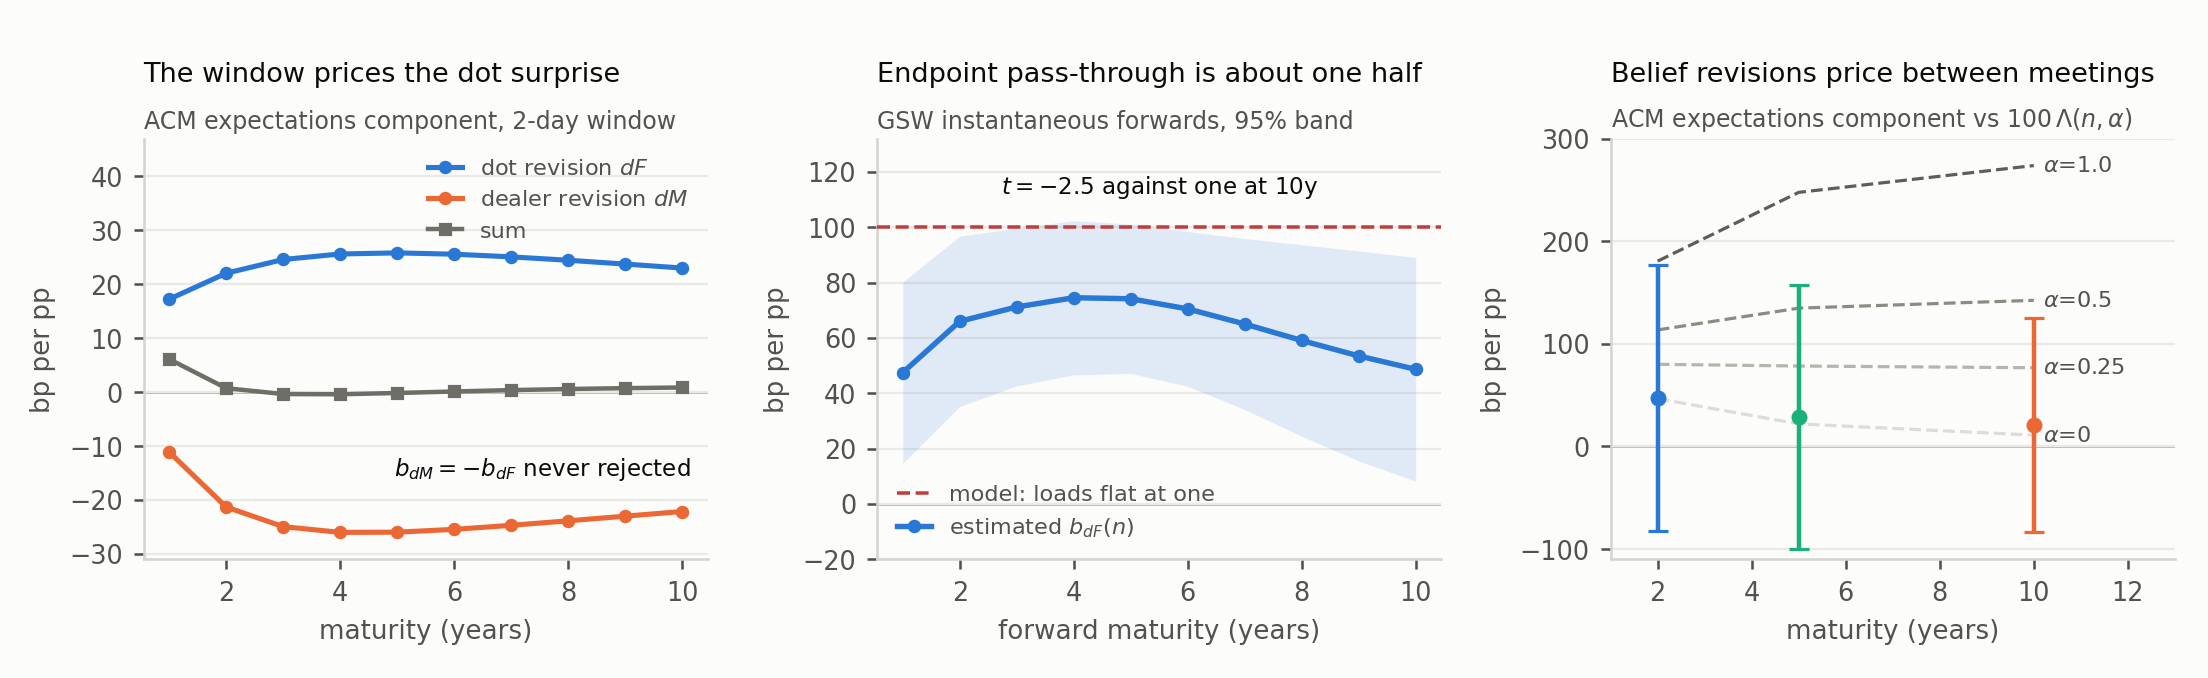
\includegraphics[width=\textwidth]{fig_tests.png}
\caption{\textbf{The dot revision and its pricing.} Left: two-day window changes in the ACM
expectations component on the dealer revision $dM$ (pre-window) and the dot revision $dF$
(in-window); the coefficients are equal and opposite, so the window prices $dF-dM$ and their sum
is zero. Centre: the dot-revision loading across GSW instantaneous forwards, 95\% bands, against
Prediction 4's flat-at-one. Right: intermeeting pricing of dealer revisions against
$100\,\Lambda(n,\alpha)$. HAC(4); 46--47 meetings.}
\label{fig:tests}
\end{figure}
\begin{figure}[tbp]
\centering
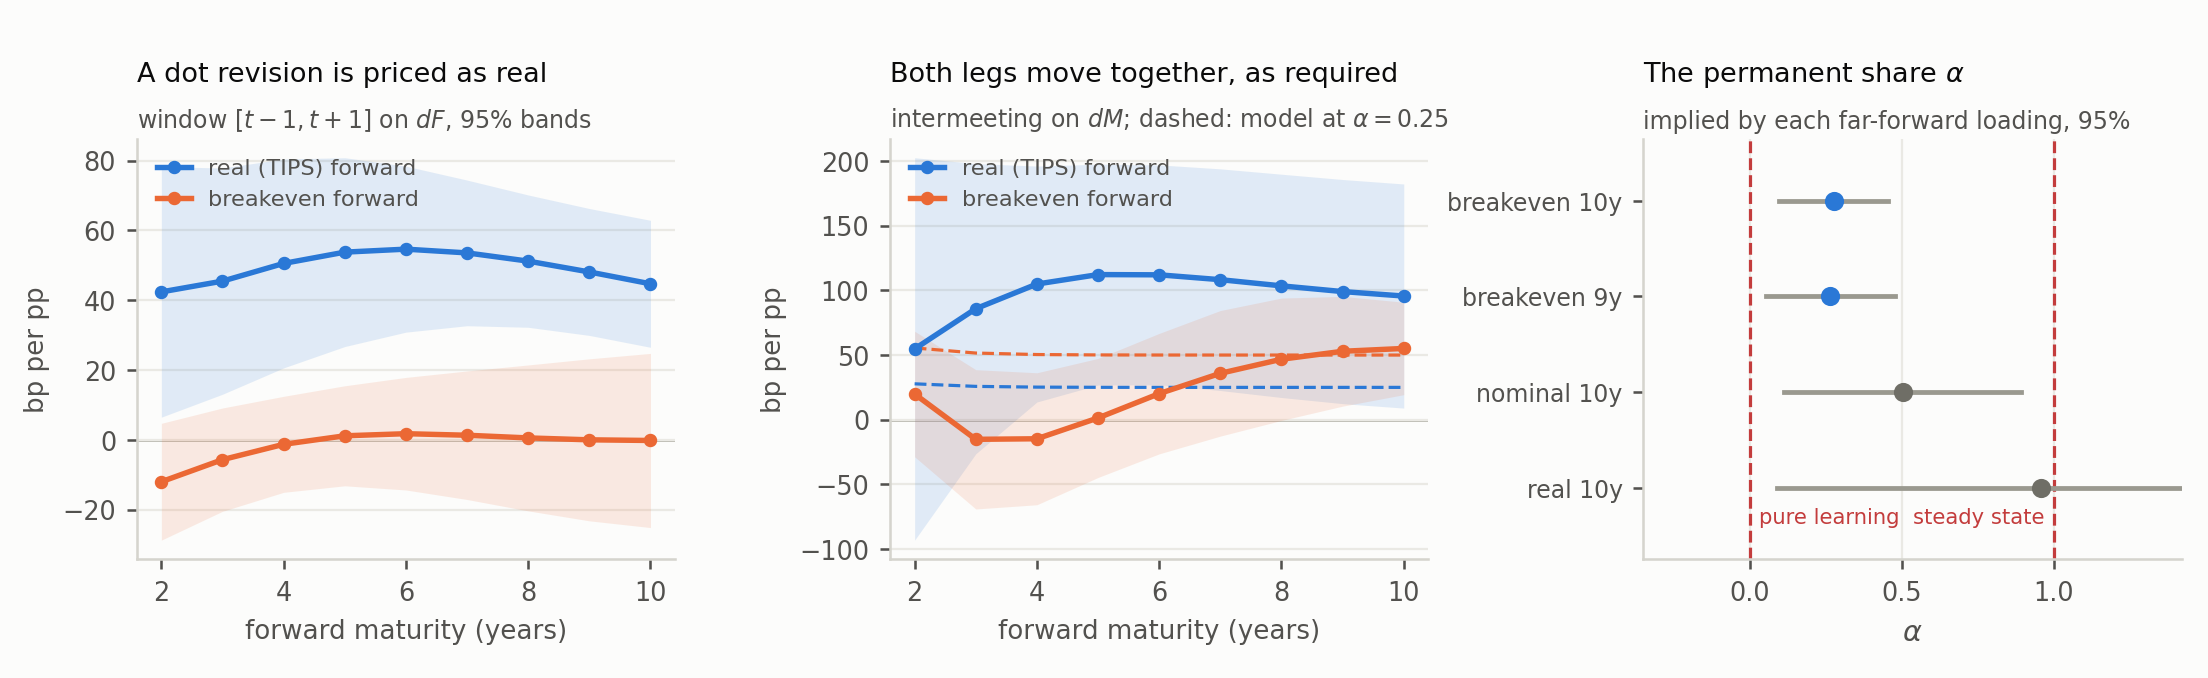
\includegraphics[width=\textwidth]{fig_tips.png}
\caption{\textbf{The composition restriction.} Left: window changes in GSW real (TIPS) and
breakeven instantaneous forwards on $dF$ --- entirely real beyond three years. Centre: the same
legs on $dM$ between meetings, model loadings at $\alpha=0.25$ dashed; both move together, as
the model requires and the window specifications do not. Right: $\alpha$ implied by each
far-forward loading, where $\lambda_{120}\to3\alpha$. HAC(4); Fieller intervals for ratios.}
\label{fig:tips}
\end{figure}
\subsection{The remaining predictions, and where this leaves the program}
\label{sec:test-rest}
\textbf{Symmetry survives.} Splitting the level response at $\delta=0$ (10y, two-day window)
gives $p$(symmetric) $=0.98$ for the total yield, $0.79$ for the expectations component and
$0.87$ for the term premium, so the linearity that distinguishes this model from Caballero \&
Simsek's sign-dependent premium is not rejected. One flag: in revisions the ten-year
term-premium response is asymmetric ($p=0.035$) --- one rejection among ten tests on 46
observations. \textbf{The premium finds nothing on the available proxy.} Against the dealers'
cross-sectional IQR of the longer-run rate, ACM term premia are flat in levels, insignificant in
changes, and show no rise with maturity --- but forecaster dispersion is dispersion \emph{within}
the market, not uncertainty about the Fed--market gap, so this removes the easy version of the
result rather than testing the prediction.
Two vulnerabilities belong in the same breath as all of the above. The intermeeting design
carrying Prediction 2 and the $\alpha$ bound cannot separate the model's mechanism from common
macro news, so an instrument for dealer belief revisions is the natural next step; and with
sd$(\Delta\delta)=0.117$ on 46 meetings, everything here concerns small revisions to a small
gap, on a sample that grows at eight observations a year.
\vspace{0.9em}
\noindent\rule{\textwidth}{0.4pt}\\[0.2em]
\scriptsize\textbf{Key references.} Bauer, Pflueger \& Sunderam (2024), \emph{QJE}. Bauer \&
Rudebusch (2020), \emph{AER}. Caballero \& Simsek (2022), \emph{AER}. Cao, Crump, Eusepi \&
Moench, FRBNY SR 934. Cho \& Williams (2026), Liberty Street Economics. Cieslak, McMahon \&
Pang, SSRN 4920858. Engstrom, FEDS 2026-026. G\"urkaynak, Sack \& Swanson (2005). G\"urkaynak,
Sack \& Wright (2007; 2010), \emph{JME}; \emph{AEJ:Macro}. Hanson,
Lucca \& Wright (2021), \emph{QJE}. Hartley (2025), Mercatus WP. Hillenbrand (2025),
\emph{RFS}. Holston, Laubach \& Williams (2017), \emph{JIE}; (2023), FRBNY SR 1063. Joslin,
Singleton \& Zhu (2011), \emph{RFS}. Kozicki \& Tinsley (2001), \emph{JME}. Lou, Pint\'er,
\"Usl\"u \& Walker, BIS WP 1232. Lucca \& Moench (2015), \emph{JF}. Orphanides (2003),
\emph{JME}. Orphanides \& Williams (2002), \emph{BPEA}. Pan \& Peng, SSRN 4764451. Swanson
(2021), \emph{JME}.
\end{document}
